\documentclass[tikz,convert={outfile=\jobname.svg}]{standalone}

\usepackage[utf8]{inputenc}     
\usepackage{amsmath}
\usepackage{amsfonts}
\usepackage[english]{babel}
\usepackage[version=3]{mhchem}
\usepackage{epstopdf}
\usepackage[justification=centering]{caption}
% \usepackage{slashbox}
\usepackage[T1]{fontenc}
\usepackage{tikz}
\usetikzlibrary{arrows} 
\usepackage{pgfplots}
\usepackage[hidelinks]{hyperref}
\usepackage{subcaption}
\usepackage[version=3]{mhchem}
\usepackage{subcaption}
\usepackage{amsthm}
\usepackage{empheq}
\usepackage{braket}
\usepackage[left=2.5cm,top=3cm,right=2.5cm,bottom=3cm,bindingoffset=0.5cm]{geometry}
\usepackage{subcaption}
\usepackage{caption}
\usepackage{listings}
% \usepackage[style=numeric]{biblatex}
% \addbibresource{biblio.bib}
\allowdisplaybreaks
\usetikzlibrary{decorations.pathmorphing}
\usetikzlibrary{decorations.markings}

\tikzset{
    every node/.append style={font=\small},
    every edge/.append style={thick},
    arrow/.style={thick, shorten >=5pt,shorten <=5pt,->},
    photon/.style={decorate, decoration={snake}},
    electron/.style={postaction={decorate},
        decoration={markings, ,mark=at position .55 with {\arrow[]{>}}}},
}
%\usetikzlibrary{...}% tikz package already loaded by 'tikz' option
\begin{document}
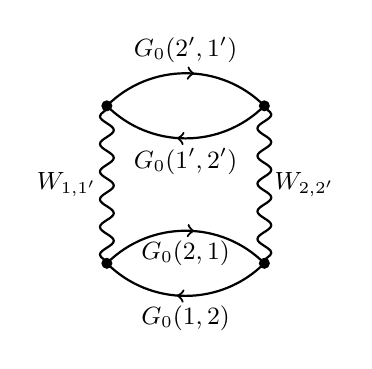
\begin{tikzpicture}[]
  \begin{scope}[scale=2]
      % coordinates
      \coordinate (in) at (-.5,0);
      \coordinate (out) at (1.5,0);
      \fill (0,0) circle (1pt) coordinate (lb);
      \fill (0,1) circle (1pt) coordinate (lt);
      \fill (1,0) circle (1pt) coordinate (rb);
      \fill (1,1) circle (1pt) coordinate (rt);

      % edges
      \draw (lb) edge[electron,out=45,in=135] node[below] {$G_0(2,1)$} (rb);
      \draw (rb) edge[electron,out=-135,in=-45] node[below] {$G_0(1,2)$} (lb);
      \draw (lt) edge[electron,out=45,in=135] node[above] {$G_0(2',1')$} (rt);
      \draw (rt) edge[electron,out=-135,in=-45] node[below] {$G_0(1',2')$} (lt);
      \draw (lb) edge[photon] node[left] {$W_{1,1'}$} (lt);
      \draw (rt) edge[photon] node[right] {$W_{2,2'}$} (rb);
  \end{scope}
\end{tikzpicture}
\end{document}